% !TeX encoding = UTF-8
\chapter{Latex-Tutorial zur Vorlage}
\label{cha:BspInhalt}
Hier gibts eine Menge Text. Zunächst eine Einführung, was denn in diesem Kapitel alles beschrieben ist. Dazu kann man vielleicht auch kurz die Resultate aus vorhergehenden Kapitel, z.B. aus Kapitel \ref{cha:Einleitung} nutzen.

Im Folgenden wird das Arbeiten mit dieser Vorlage näher erläutert und Tipps gegeben, die den Einstieg in das Arbeiten mit Latex erleichtern sollen. Es wird empfohlen den Latex Editor Texstudio mit MikTex zu verwenden (Miktex muss zuerst installiert werden). Mit diesem Editor ist es möglich das Hauptdokument \fe{studentische\_arbeit\_main.tex} explizit als root-Dokument festzulegen. Anschließend kann der Kompilierungsvorgang ausgehend von jedem beliebigen Teildokument gestartet werden. Bei der ersten Kompilierung des Hauptdokuments wird, bei Verwendung eines geeigneten Editors, nach der Vertrauenswürdigkeit des Dokuments gefragt. Diese Frage ist zu bejahen, da wichtige Argumente durch \fe{Magic Comments} im Dokument \fe{studentische\_arbeit\_main.tex} zu den Standardbefehlen des Editors hinzugefügt werden. 

Wenn ein anderer Texeditor (z.B. TeXnicCenter) verwendet werden soll, müssen bestimmte Einstellungen in den Editoroptionen vorgenommen werden (Siehe \cite{schubert.2014} und \cite{kurt.2014}).

Die Generierung des folgenden Inhalt kann auch im zugehörigen Quellcode im Tex-Dokument nachvollzogen werden.

Als Erstes sollte die Datei \fe{myData.tex} ausgefüllt werden.

\section{Symbolverzeichnis}\label{subsec:notation}
Zur Erstellung von Verzeichnissen wird das \fe{glossaries} Package empfohlen. Dieses erfordert die Ausführung des Befehls \fe{makeglossaries}, welcher wiederum die Installation von \fe{Perl (z.B. ActivePerl)} erfordert. Im root-Dokument wurde mithilfe von \fe{Magic-Comments} eine sinnvolle Befehlsabfolge festgelegt. Um das Symbolverzeichnis anzupassen muss die Datei \fe{notation.tex} bearbeitet werden. Dort können Einträge mit
\begin{lstlisting}[style=myLatexStyle]
	\newglossaryentry{refkey}{name=Symbolname,
	description={Beschriebungstext},
	unit={\si{\einheit}},
	type=symbolslist}	
	\end{lstlisting}
eingefügt werden.
Anschließend wird beim (evtl. mehrmaligem) Kompilieren das Symbolverzeichnis erstellt. Die Symbole können mit  
\lstinline|\gls{refkey}| referenziert werden.
\section{Abkürzungen}
Es können Abkürzungen, wie z.B. \gls{EA}, die im Abkürzungsverzeichnis (siehe \fe{notation.tex}) definiert wurden, mit \lstinline|\gls{EA}| referenziert werden 
\section{Einbindung von Grafiken}
Meistens sind auch ein paar Bildchen ganz hübsch, wenn die Bildchen selbst ganz hübsch sind. Eingebunden werden sie am besten in einer gleitenden Umgebung als Vektorgrafik (.pdf für pdfLaTeX).

Dies sieht einfach besser aus, als wenn man so verpixelte Linien und Buchstaben hat. Wichtig ist, dass alle Linien dick genug sind und auch die Größe des Textes zumindest ungefähr der Textgröße in den Absätzen entspricht. Die Schriftart sollte in jedem Fall angepasst werden. Man sollte gerade auch bei Matlab-Exporten darüber nachdenken, die Standardfarben zu ändern und stattdessen die Farben aus der "`HNI-Palette"' zu verwenden. Bei Fotos wie in Bild \ref{fig:surf} hat man solche Probleme natürlich nicht.
\begin{figure}[htb]
	\centering
	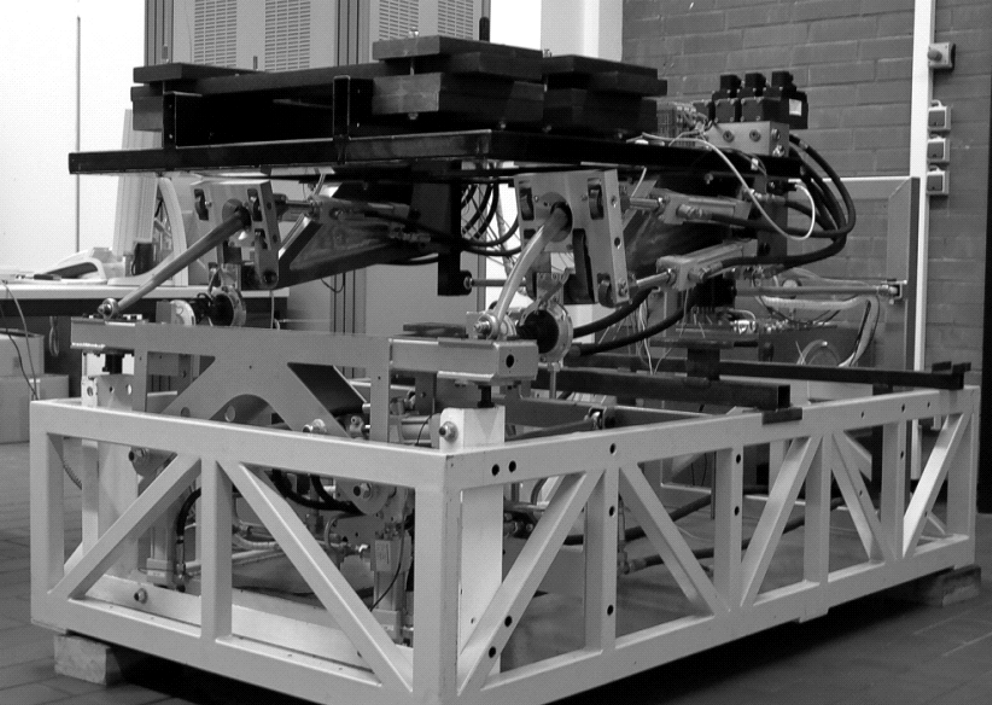
\includegraphics[width=0.7\textwidth]{Bilder/kapitel1/Pruefstand_Foto}
	\caption{Der SUrF-Prüfstand steht in unserem Labor, besteht aus ganz vielen Einzelteilen und ist ein spannendes Forschungsobjekt, vor allem aber ist dies nun eine Bildunterschrift über mehrere Zeilen.}
	\label{fig:surf}
\end{figure}

Beim Einbinden der Grafiken sollten absolute Pfade (C:/Dokumente und Einstellungen/ ... /Arbeit/Doku/Bilder/Bild1.pdf) vermieden werden. TeX kann mit relativen Pfaden umgehen (Bilder/Bild1.pdf). Damit ist sichergestellt, dass das Dokument jederzeit auch auf einem anderen Computer erstellt werden kann. Es kann sogar der Pfad eingestellt werden, in dem nach Grafiken gesucht wird. Dies geschieht in der Präambel mit \begin{lstlisting}[style=myLatexStyle]
	\graphicspath{{Bilder/kapitel1/},{...}}
\end{lstlisting}


Eine sehr schöne Möglichkeit um z.B. Matlab-Plots zu integrieren ist es, das \fe{pgfplots}-Package in Kombination mit der Matlabfunktion \fe{Matlab2tikz} (s. Dokumentenverzeichnis) zu verwenden. Dabei wird die figure in Matlab durch Aufrufen von 

ea\begin{lstlisting}[style=Matlab-editor]
	matlab2tikz('dateiname','width','\figurewidth','height','\figureheight')
\end{lstlisting}
 in eine \fe{.tex}-Datei mit den Dateinamen \fe{dateiname} und eine gespeichert. Sowohl die Text- als auch die Bildinformationen werden in der \fe{tex}-Datei hinterlegt und können mit einem Texeditor bearbeitet werden. Die Dateien können anschließend an passender Stelle mit dem Befehl \fe{$\backslash$ inserttikz} eingefügt werden. Die Befehlsreferenz
\begin{lstlisting}[style=myLatexStyle]
	\inserttikz{pfad/dateiname}{label}{caption}{Höhe}{Breite}{Pos}
	z.B 
	\inserttikz{Bilder/kapitel1/bspbild}{labeltest}{Testbild}{0.5\textwidth}{0.75\textwidth}{htbp}
\end{lstlisting}
führt auf das in Bild \ref{fig:gross} dargestellte Ergebnis. Möchte man das Bild nun verkleinert darstellen (s. \ref{fig:klein}) bleiben die Beschriftungen im passenden Schrifttyp und -größe.

\inserttikz{Bilder/kapitel1/bspbild}{fig:gross}{Bild wurde in Matlab generiert und mit \fe{matlab2tikz} exportiert}{0.4\textwidth}{0.7\textwidth}{htbp}

\inserttikz{Bilder/kapitel1/bspbild}{fig:klein}{Verkleinerte Version des zuvor eingefügten Bildes. Die Beschriftungen bleiben dennoch in einer leserlichen Größe}{0.2\textwidth}{0.5\textwidth}{htbp}
\clearpage
\subsection{Gleichungen}
Manchmal ist es aber mit Text nicht getan, dann ist unter Umständen eine Formel besser. Aber Achtung, Formeln sollten immer in den Text eingebunden werden und niemals für sich alleine stehen. Beispielsweise beschreiben die beiden Gleichungen 
\begin{es}
\label{eq:LTIsys} 
\dot{\vec{x}}(t) &= \vec{A}\vec{x}(t) + \vec{B}\vec{u}(t) \\
\vec{y}(t) &= \vec{C} \vec{x}(t)
\end{es}

mit	\begin{es}
	A & = ...\\
	B & = ...\\
	...
	\end{es}
ein lineares dynamisches System. Vektoren und Matrizen sollten mit dem Befehl \fe{\textbackslash vec\{\}} markiert werden. Die Gleichung \eqref{eq:LTIsys} ist außerdem ein Beispiel dafür, dass beide Gleichungen nur eine gemeinsame Formelnummer besitzen. Es bietet sich dafür an die Umgebung \fe{es} dafür benutzt werden. Es handelt sich dabei eine Kombination aus den Umgebungen \fe{align} und \fe{equation}.

Erst wenn man Gleichung \eqref{eq:LTIsys} mit \fe{eqref} referenziert, wird diese nummeriert! Dadurch wird vermieden, dass der Formelzähler unnötig groß wird.

Steht eine Formel am Ende eines Satzes, so ist ein Punkt innerhalb der Formelumgebung zu setzen, beispielsweise bei dieser Formel
\begin{equation}  
\label{eq:RiccatiJ}
J(x(t), u(t)) = \frac{1}{2} \int_0^\infty x(t)^T Q x(t) + u(t)^T S u(t) \ dt. 
\end{equation}
Hier beginnt dann ganz korrekt der neue Satz. Da auch die Gleichung \eqref{eq:RiccatiJ} eine wichtige Gleichung ist, die noch einmal referenziert wird, besitzt sie eine Formelnummer.

Mitunter muss man sogar Matrizen in der Arbeit angeben. Dazu ist es ganz praktikabel entsprechende Befehle zu verwenden und nicht selbst irgendetwas zusammen zu bauen. Es gibt sowohl Matrizen mit eckigen Klammer
\begin{equation}
\begin{bmatrix} A_{11} & A_{12} \\ A_{21} & A_{22} \end{bmatrix},
\end{equation}
als auch welche mit runden Klammern
\begin{equation*}
\begin{pmatrix} A_{11} & A_{12} \\ A_{21} & A_{22} \end{pmatrix}.
\end{equation*}

Mitunter fällt einem dann ein, dass an manchen Stellen noch etwas zu verbessern ist, aber man hat gerade keine Zeit oder keine Lust. Damit man seinen Gedankenblitz dann nicht so schnell vergisst, kann man den Befehl \fe{todo\{\}} zur graphischen Hervorhebung benutzen:
\todo{Dieser Absatz muss noch viel besser werden!}


Wenn Zahlen und Einheiten benötigt werden sollte das Paket \fe{siunitx} benutzt werden. Es ist in diesem Dokument so konfiguriert, dass es bei Zahlen immer ein Komma verwendet. 

\begin{itemize}
	\item\text{Einheit und Zahl} 
	\begin{lstlisting}[style=myLatexStyle]
	g=\SI{9.81}{\meter\per\square\second}
	\end{lstlisting} produziert die Ausgabe $g=\SI{9.81}{\meter\per\square\second}$\\
	\item\text{nur Zahl} 
	\begin{lstlisting}[style=myLatexStyle]
	\num{9.81}
	\end{lstlisting} produziert die Ausgabe $\num{9.81}$\\
	\item\text{nur Einheit} 
	\begin{lstlisting}[style=myLatexStyle]
	\si{\meter\per\square\second}
	\end{lstlisting} produziert die Ausgabe $\si{\meter\per\square\second}$
\end{itemize}
	
\subsection{Beispieltabellen}
Ansehnliche Tabellen lassen sich mit \fe{tabularx} und \fe{booktabs} erstellen. Die jeweiligen Spaltenbreiten lassen sich prozentual festlegen. Verwendet man eine "X"-Spalte ist der automatische Zeilenumbruch aktiviert.

Der Latex-Code
\begin{lstlisting}[style=myLatexStyle]
	\begin{table}[htbp] \caption{Mechanische Parameter des Doppelpendels auf einem Wagen}\label{tab:bsp}
	\begin{tabularx}{\linewidth}{
	>{\setlength\hsize{0.5\hsize}}X% 1.Spalte
	>{\setlength\hsize{0.25\hsize}}X% 2.Spalte
	>{\setlength\hsize{0.25\hsize}}X% 3.Spalte
	} 
	\toprule
	& innerer Pendelarm & äußerer Pendelarm\\
	& $i=1$ & $i=2$ \\ 
	\midrule
	Länge $l_i$ [\si{\meter}] & \num{0.356} & \num{0.356} \\
	Abstand zum Schwerpunkt $a_i$ [\si{\meter}]& \num{0.18} & \num{0.148} \\
	Masse $m_i$ [\si{\kilogram}] & \num{0.775} & \num{0.654} \\
	Trägheitsmoment $J_i$ [\si{\newton\meter\square\second}] & \num{0.0224} &\num{0.0179} \\
	Dämpfungskonstante $d_i$ [\si{\meter}] & \num{0.005} & \num{0.005} \\ 
	\bottomrule
	\end{tabularx}
	\end{table}
\end{lstlisting}
produziert die Tabelle \ref{tab:bsp}
\begin{table}[htbp] \caption{Mechanische Parameter des Doppelpendels auf einem Wagen}\label{tab:bsp}
	\begin{tabularx}{\linewidth}{
			>{\setlength\hsize{0.4\hsize}}X% 1.Spalte
			>{\setlength\hsize{0.3\hsize}}X% 2.Spalte
			>{\setlength\hsize{0.3\hsize}}X% 3.Spalte
		} 
		\toprule
		& innerer Pendelarm & äußerer Pendelarm\\
		& $i=1$ & $i=2$ \\ 
		\midrule
		Länge $l_i$ [\si{\meter}] & \num{0.356} & \num{0.356} \\
		Abstand zum Schwerpunkt $a_i$ [\si{\meter}]& \num{0.18} & \num{0.148} \\
		Masse $m_i$ [\si{\kilogram}] & \num{0.775} & \num{0.654} \\
		Trägheitsmoment $J_i$ [\si{\newton\meter\square\second}] & \num{0.0224} &\num{0.0179} \\
		Dämpfungskonstante $d_i$ [\si{\meter}] & \num{0.005} & \num{0.005} \\ 
		\bottomrule
	\end{tabularx}
\end{table}